
\section{Word2Vec}
\label{sec:w2v}

Word2Vec is an unsupervised learning algorithm published in 2013, which, based
on a corpus of text, provides a vector representation for each word of that
text, using a two-layer neural network. This algorithm was initially implemented
to learn word representations from large data sets efficiently but emerged as a
standard embedding technique. According to the use case, two models are
available: Continuous Bag-Of-Words (CBOW) and Skip-Gram (SG).

\subsection{Continuous Bag-of-Words Model}
\label{subsec:w2v:cbow}

CBOW is an unsupervised model that predicts a target word based on context words
and window size. From a semantic point of view, the model is named
``Bag-of-Words'' since the order of the context words does not influence its
training.
\begin{figure}[!ht]
  \centering
  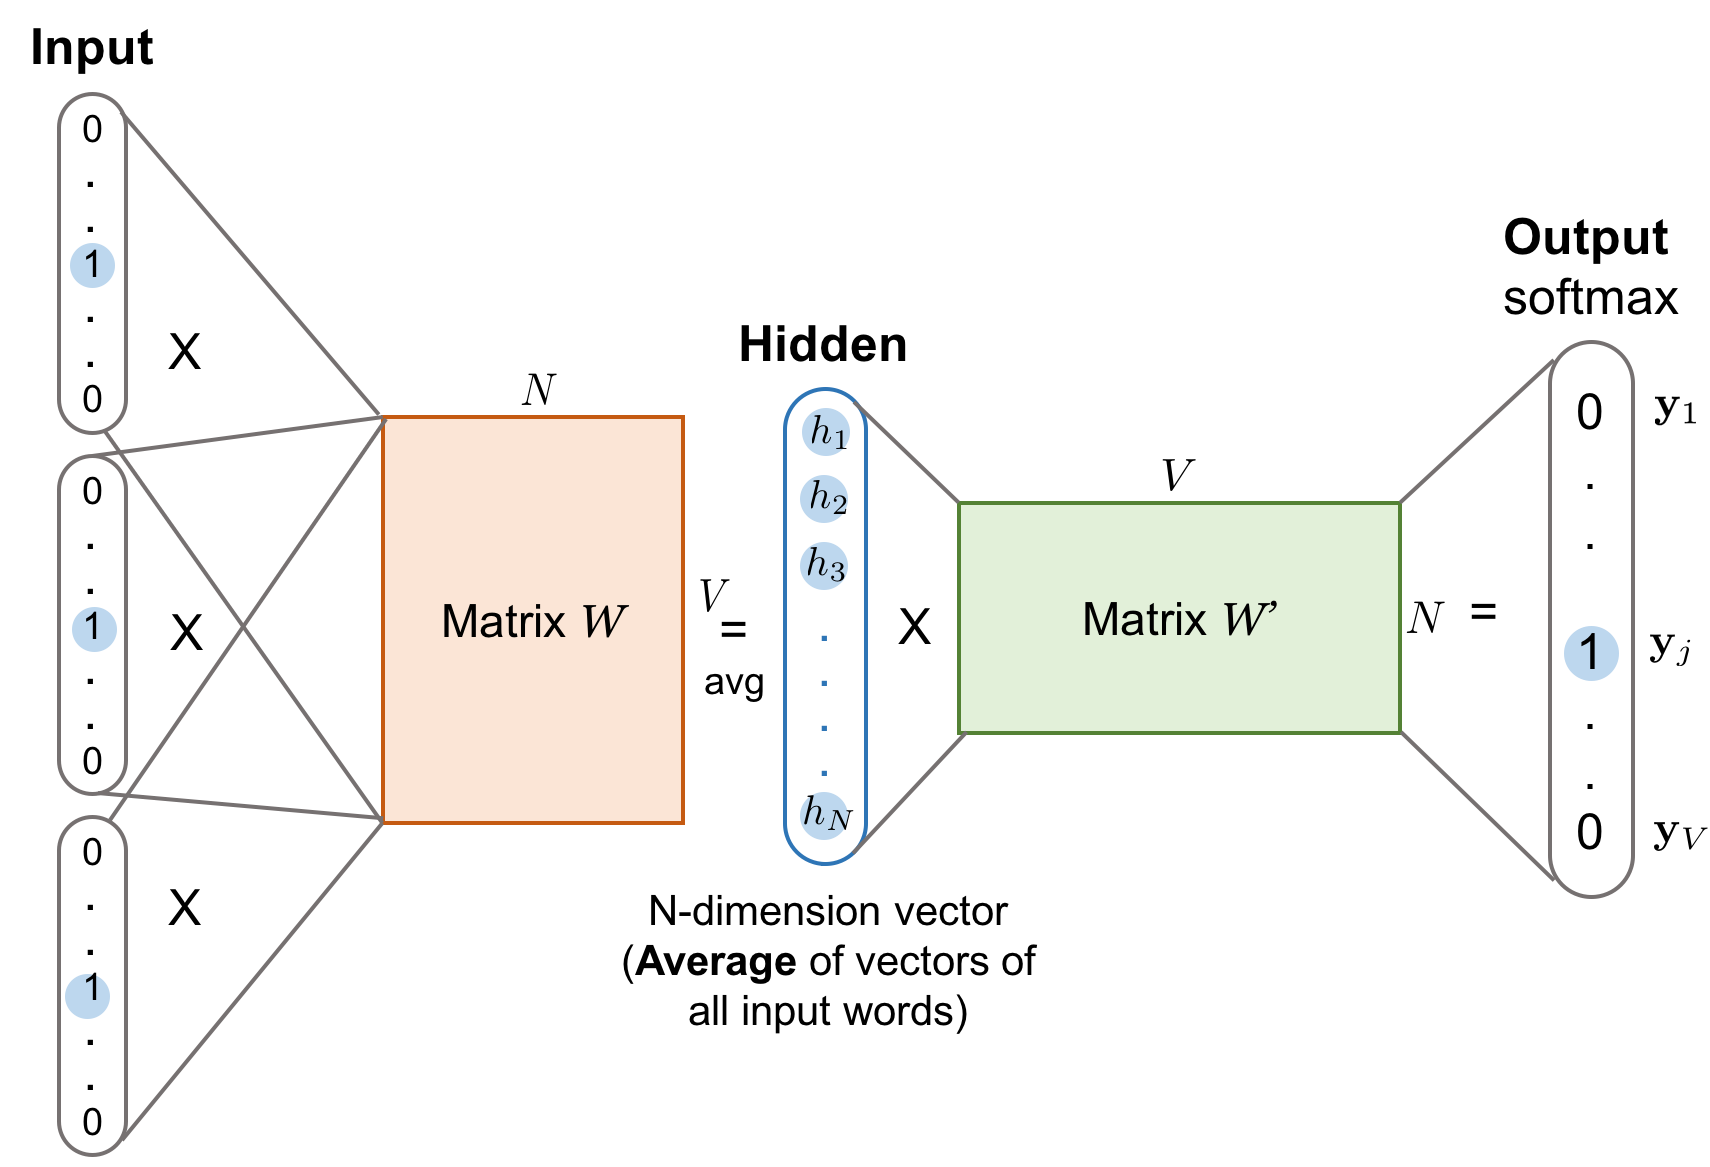
\includegraphics[width=0.75\textwidth]{img/embedders/w2v/cbow}
  \caption{CBOW Model Architecture.}
  \source{
    \href{https://lilianweng.github.io/lil-log/2017/10/15/learning-word-embedding.html}
    {Lilian Weng -- Learning Word Embedding}
  }
  \label{fig:w2v:cbow:architecture}
\end{figure}

In Figure \ref{fig:w2v:cbow:architecture}, the CBOW model architecture starts by
taking one or several targets word as input, represented as a $V$-dimensional
one-hot encoding vector. $V$ is the dictionary's size of unique words present in
a text or in a training data set. Using a dot product, this/these input
vector(s) is then multiplied by a first $W$ weight matrix, named embedding
matrix. This matrix is of dimension $V \times N$, where $N$ is the number of
features that each unique word in this vocabulary has defining the
\emph{embedding size}. Therefore, these dot products produce an $N$-dimensional
hidden vector for each input vector. However, if there multiple input context
vectors, these hidden vectors are then averaged element-wise into a single
hidden vector, where this vector chooses the size of the vectors that will be
used later.

According to the semantics of the words of the dictionary, a new dot product is
made, but this time, between the calculated hidden vector and another $W'$
weight matrix, named \emph{context matrix}. This matrix being now of dimension
$N \times V$. Then, their product generates an output vector of dimension $V$
subjected to a softmax activation function. Therefore, this function ends by
calculating a probability distribution and returns the probability that a word
is a target word for the given context words. Finally, a cross-entropy loss
function is applied to compute the loss between the true probability
distribution of the given target word and the calculated model probability.

\begin{definition}[Cross-Entropy]
  Measures the difference between two probability distributions for a given
  random variable. Let $p$ be a true probability distribution, $q$ be a computed
  model probability, and $c$ be the predicted result by an ML
  algorithm. Mathematically, the cross-entropy loss can be defined as follows:
  \begin{equation}
    H(p, q) = -\sum_{c=1}^Cp(c)\log\left(q(c)\right)
    \label{eq:cross-entropy}
  \end{equation}
  \label{def:cross-entropy}
\end{definition}

After computation with the cross-entropy loss, the back-propagation updates the
weights of the embedding matrix according to this loss. These steps are then
repeated with other context words and another target word for a specified number
of epochs. Once the training is done, the embedding matrix is used to generate
the word embeddings from the one-hot encodings. Formally, given a sequence of
training words $w_1, w_2, \dotsc, w_t$, and a context window $c$, the objective
of the CBOW model is to maximize the average log probability:
\begin{equation}
  \frac{1}{T}\sum_{t=1}^T\log\left(p\left(w_t|w_{t-c}, \ldots, w_{t + c}\right)\right)
  \label{eq:w2v:cbow:probability}
\end{equation}

where $T$ is the number of training samples, and the probability
$p\left(w_t|w_{t-c}, \ldots, w_{t + c}\right)$ is computed using the softmax
function (cf. Definition \ref{def:softmax}):
\begin{equation}
  p\left(w_t|w_{t-c}, \ldots, w_{t + c}\right) =
  \frac{\exp\left(v^{-T}v'_{w_t}\right)}{\sum_{w=1}^W\exp\left(v^{-T}v'_w\right)}
  \label{eq:w2v:cbow:probability:details}
\end{equation}

where $W$ is the vocabulary size, $v'_w$ is the output vector of the $w$ word,
and $v$ is the averaged input vector of all the context words:
\begin{equation}
  \overline{w}_t = \frac{1}{2c}\sum_{-c\leq j \leq c,j \neq 0}w_{t + j}
  \label{eq:w2v:cbow:probability:details2}
\end{equation}

\noindent Finally, the whole network is not used regarding the generation of embeddings,
but only its first layer.

\subsection{Skip-Gram Model}
\label{subsec:w2v:sg}

SG is an unsupervised model that predicts context words from a target word,
according to window size and a sentence. Unlike CBOW, these context words are
defined as multiple pairs of words (cf. Table \ref{def:window:size}), serving as
training samples for this model. Such training allows this model to learn word
vector representations suitable for predicting nearby words within a text,
except for common words and stop words (cf. Section
\ref{subsec:w2v:sfw}). Finally, SG compresses the information in a low
dimensional space, such that this model learns a continuous low dimensional
representation for the words.

The window size for each target word is arbitrarily chosen between one and a
small positive number. This choice allows to add randomness during training and
improves future predictions. In the case of a window size greater than two, the
context words for a target word likely are more than two. If such a situation
occurs, SG randomly picks a word from these word contexts to form a pair with
the context word. Then, this model counts the number of times this pair of words
appear, and the model starts to be trained.

Similar to CBOW, given a sequence of target words $w_1, w_2, \ldots, w_t$, and a
context window $c$, the objective of the SG model is to maximize the average log
probability:
\begin{equation}
  \frac{1}{T}\sum_{t=1}^T\sum_{-c \leq j \leq c, j \neq 0}\log\left(p\left(w_{t+j}|w_t\right)\right)
  \label{eq:w2v:sg:probability}
\end{equation}

where $T$ is the number of training samples, and the probability $p\left(w_{t +
j}|w_t\right)$ is also computed using the softmax function (cf. Definition
\ref{def:softmax}):
\begin{equation}
  p\left(w_o|w_i\right) = \frac{\exp\left(u_{w_o}^Tv_{w_i}\right)}{\sum_{w=1}^W\exp\left(u_w^Tv_{w_i}\right)}
  \label{eq:w2v:sg:probability:details}
\end{equation}
where $W$ is the vocabulary size, $v$ the input representation of a word, and
$u$ the output representation of a word.

\begin{figure}[!ht]
  \centering
  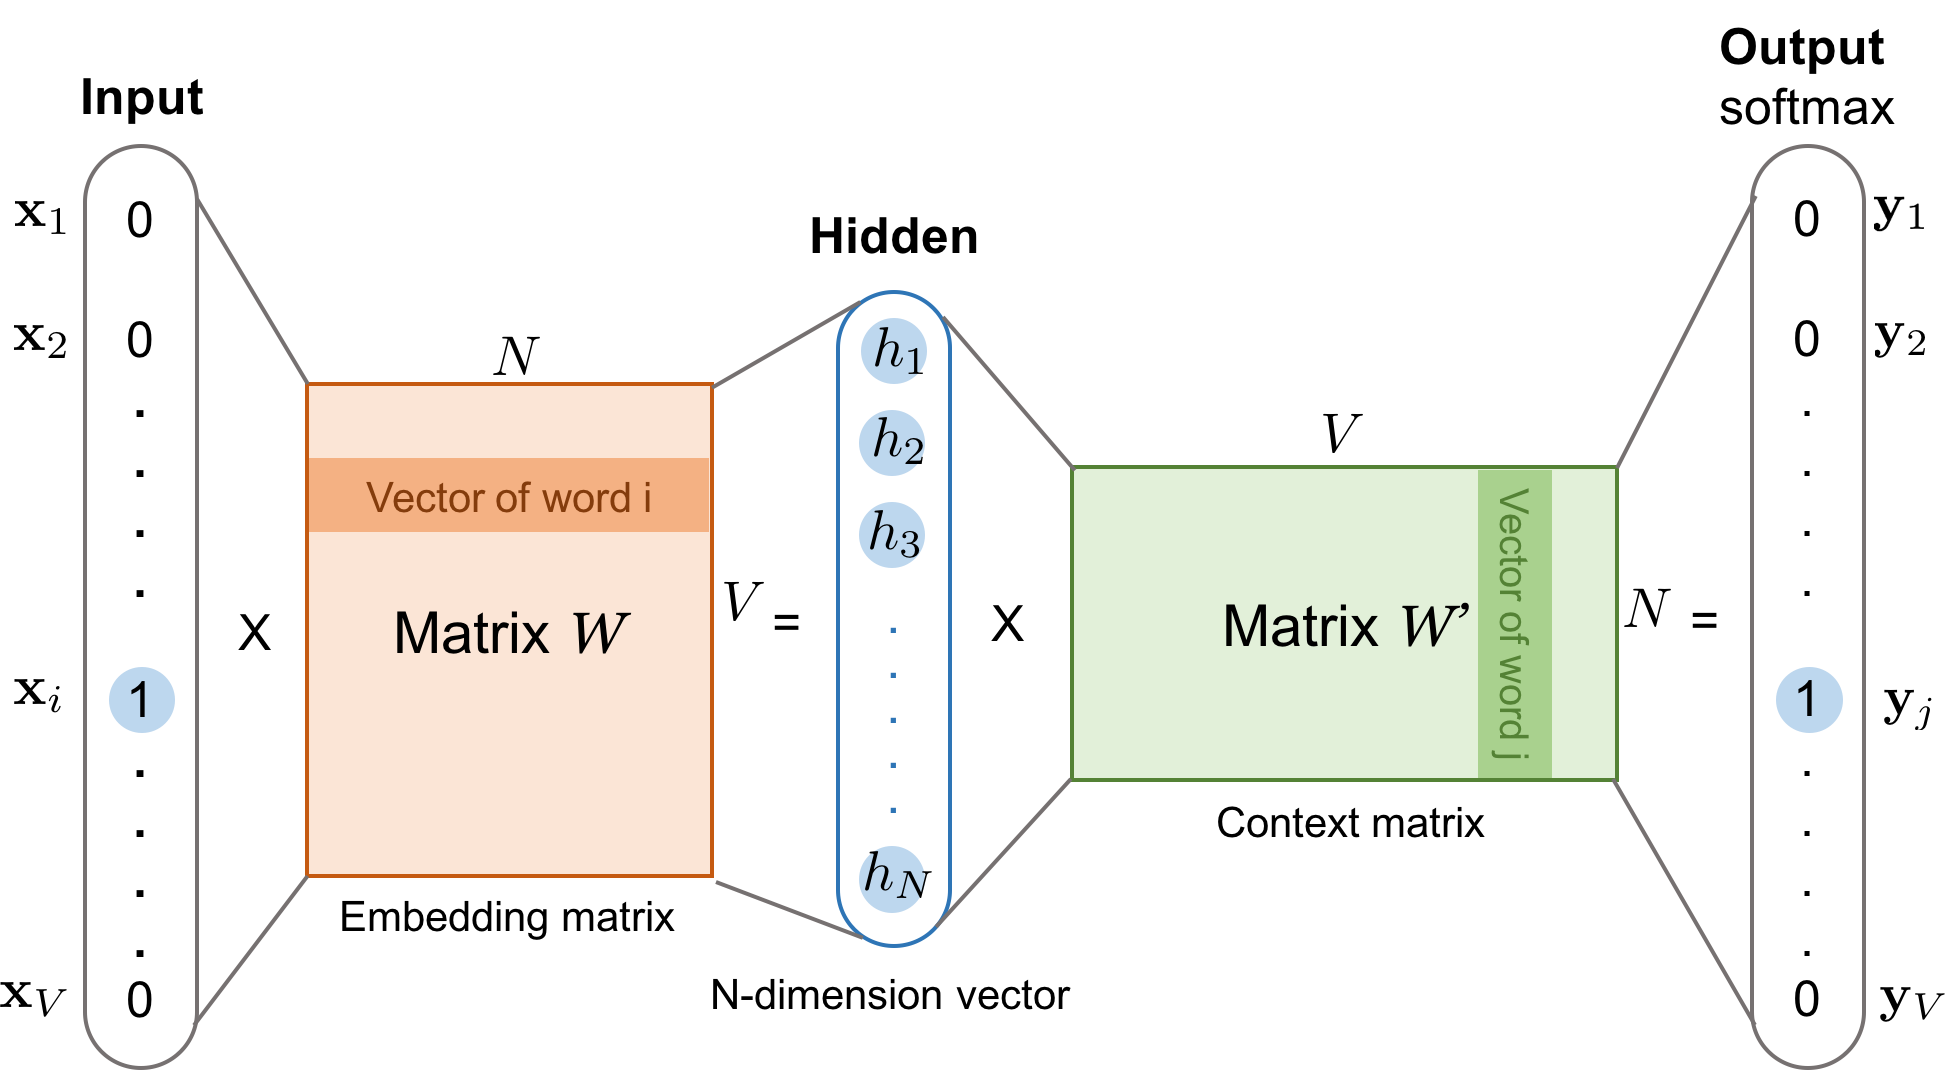
\includegraphics[width=0.8\textwidth]{img/embedders/w2v/skip-gram}
  \caption{SG Model Architecture.}
  \source{
    \href{https://lilianweng.github.io/lil-log/2017/10/15/learning-word-embedding.html}
    {Lilian Weng -- Learning Word Embedding}
  }
  \label{fig:w2v:sg:architecture}
\end{figure}

In Figure \ref{fig:w2v:sg:architecture}, the SG model architecture can be seen
as the inverse of the CBOW architecture. With this architecture, instead of
having context words and predicting a target word, it takes two words. From then
on, a model will predict a target word according to a context word. In addition,
since there is only one input word, the embedding matrix directly generates a
hidden layer with no need to do an average. Finally, the cross-entropy loss
function is applied this time to compute the loss between the true probability
distribution of the given context word and the calculated model probability.

\subsection{Subsampling Frequent Words}
\label{subsec:w2v:sfw}

Subsampling frequent words is a technique whose objective is to reduce the
number of training examples for a Word2Vec model. To accomplish this, it assumes
that predicting context words that are too frequent (e.g., ``the'') provides
little semantic value to differentiate a context
~\citep{inproceedings:mikolov}. In contrast, infrequent words are more likely to
convey specific information. Therefore, to improve the balance between
infrequent and frequents words, this technique randomly eliminates words from a
more frequent corpus than a certain threshold. This suppression occurs before a
corpus is processed in word-context pairs.

Let $w_i$ be a word, $f_{w_i}$ be a word frequency in a corpus, and $t$ be a
chosen threshold, typically around $10^{-5}$. Mathematically, the discarding of
a word from a corpus is done as follows:
\begin{equation}
  P(w_i) = 1 - \sqrt{\frac{t}{f(w_i)}}
  \label{eq:w2v:sfw}
\end{equation}

Therefore, each word $w_i$ present in a text for a window of size $c$ has a
probability of being deleted, where each deleted word reduces the training
samples by most $c$ times. Therefore, words whose frequency is above this
threshold, will be aggressively subsampled, preserving the frequency
ranking. However, even though this formula speeds up learning and even
significantly improves the accuracy of learned vectors of infrequent
words~\citep{inproceedings:mikolov}, the Word2Vec implementation uses another
more elaborate formula to discard a word:
\begin{equation}
  P(w_i) = \left(\sqrt{\frac{z(w_i)}{t}} + 1\right)\frac{t}{z(w_i)}
  \label{eq:w2v:sfw:real}
\end{equation}

where $t$ has a default threshold of $10^{-3}$ and $z(w_i)$ is the fraction of
the total words in the corpus that corresponds to this word. For example, if the
``cat'' word occurs 1000 times in a billion words corpus, then $z($``cat''$) =
10^{-6}$. Therefore, $P(w_i) = 1$ when $z(w_i) \leq 0.0032z(w_i) \leq 0.0032$
means to keep every instance of a word that represented \SI{0.32}{\percent} or
less and subsampled those that have a higher percentage. Please note that
$P(w_i)$ does not correspond to a probability since it is no longer bounded
between 0 and 1. Finally, from the accuracy point of view, subsampling frequent
words can improve some accuracy and decrease one of the others.

\subsection{Hierarchical Softmax}
\label{subsec:w2v:hsm}

Hierarchical Softmax (HSM) is an efficient softmax approximation technique that
uses a multilayer binary tree structure to reduce the computational cost of
training a softmax neural network~\citep{DBLP:conf/aistats/MorinB05}. In this
data structure, each node without child nodes, called \emph{leaf nodes},
corresponds to a word and each internal node stands for relative probabilities
of the children nodes.

For better accuracy, HSM structures the Word2Vec vocabulary using a
\textsc{Huffman} tree, a binary tree data structure where data is stored in leaf
nodes, without any particular order. To structure this vocabulary, HSM uses this
tree so that frequent words are closer to the root node of the tree while
infrequent words are deeper in this tree. Therefore, more frequent words have a
greater weight than infrequent words, where the \emph{path length} is
proportional to the frequency of a word. The path length of a tree is defined as
the number of nodes that must be traversed to reach a specific
word. Consequently, a \textsc{Huffman} tree always has $n$ leaf nodes for $n-1$
internal nodes, where each node is characterized by a weight defined by a
numerical identifier. As a result, the weight of each parent node is equal to
the sum of the lower weights of its children.

To compute the probability distribution of reaching a word, HSM uses a sigmoid
activation function and two matrices. One for the inputs and one for the outputs
differ on the values stored in each row.
\begin{table}[!ht]
  \centering
  \begin{subtable}[b]{0.5\textwidth}
    \centering
    \begin{tabular}{cc}
      \toprule
      \textbf{Target Word} & \textbf{Context Words} \\
      \midrule
      \dots & \dots, \dots \\
      sleep & sleep, cat \\
      \bottomrule
    \end{tabular}
    \caption{Input Matrix}
  \end{subtable}%
  \begin{subtable}[b]{0.5\textwidth}
    \centering
    \begin{tabular}{ccc}
      \toprule
      \textbf{Node} & \textbf{Sigmoid Value} &  \textbf{Label} \\
      \midrule
      \dots & \dots & \dots \\
      14 & 0.84 & 1 \\
      20 & 0.23 & 0 \\
      \bottomrule
    \end{tabular}
    \caption{Output Matrix}
  \end{subtable}
  \caption{HSM Matrices for the SG Model.}
  \label{fig:w2v:hsm:matrices}
\end{table}

In Table \ref{fig:w2v:hsm:matrices}, the input matrix of a SG model contains
training samples for different target words. On the other hand, the output
matrix has rows of node weights related to labels and a probability determined
by the sigmoid function. This label, which can only have two values (zero or
one), helps informs navigation in the tree based on a node. By convention, zero
means to browse the left branch of this tree and one, the other
branch. Therefore, the output matrix reports that the ``cat'' context word is
found for the ``sleep'' target word by turning left at node 20 and turning right
at node 14.

\begin{figure}[!ht]
  \centering
  \resizebox{0.6\textwidth}{!}{%
    \begin{tikzpicture}
      \node[entity,minimum size=0.9cm,fill=myblue] (node_20) at (0,0) {20};

      \node[entity,minimum size=0.9cm,fill=myblue] (node_14) at (-2.5,-1) {14};
      \node[entity,minimum size=0.9cm,fill=myblue] (node_6) at (2.5,-1) {6};

      \node[entity,minimum size=0.9cm,fill=myblue] (node_dog) at (-4,-2.5) {8};
      \node[circle,draw,fill=myred] (node_cat) at (-1,-2.5) {9};

      \node[entity,minimum size=0.9cm,fill=myblue] (node_rabbit) at (1,-2.5) {4};
      \node[entity,minimum size=0.9cm,fill=myblue] (node_2) at (4,-2.5) {2};

      \node[entity,minimum size=0.9cm,fill=myblue] (node_horse) at (2.5,-4) {1};
      \node[entity,minimum size=0.9cm,fill=myblue] (node_fish) at (5.5,-4) {1};

      \draw[color=red,text=black] (node_20) -- (node_14) node[edge] {\textcolor{red}{0}};
      \draw (node_20) -- (node_6) node[edge] {1};

      \draw[color=red,text=black] (node_14) -- (node_cat) node[edge] {\textcolor{red}{1}};
      \draw (node_14) -- (node_dog) node[edge] {0};

      \draw (node_6) -- (node_rabbit) node[edge] {0};
      \draw (node_6) -- (node_2) node[edge] {1};

      \draw (node_2) -- (node_horse) node[edge] {0};
      \draw (node_2) -- (node_fish) node[edge] {1};

      \node[label,below of=node_cat] {\textcolor{red}{\textbf{cat}}};
      \node[label,below of=node_dog] {dog};
      \node[label,below of=node_rabbit] {rabbit};
      \node[label,below of=node_horse] {horse};
      \node[label,below of=node_fish] {fish};
    \end{tikzpicture}
    }%
  \caption{\textsc{Huffman} Tree for Word2Vec.}
  \label{fig:w2v:hsm:huffman}
\end{figure}

In Figure \ref{fig:w2v:hsm:huffman}, a vocabulary of five words is structured in a
\textsc{Huffman} tree containing four internal nodes, where each edge indicates a
label. This training aims to teach the model to navigate in the tree by finding
a context word based on a target word. For this search, the tree is traversed
from top to bottom, where HSM does the dot product between the target word
vector and the current node. Afterward, the result is sent to a sigmoid
activation function which returns a probability value. According to this value,
HSM checks that this probability is correct based on a label and updates the
neurons' weights if needed. This process is repeated until the word context for
a target word is found. Since training is not done on all words, there is no
need to traverse every tree node. As a result, the complexity of the gradient
goes from $\mathcal{O}(W)$ to $\mathcal{O}(\log_2(w))$. Once the training is
completed, the SG model (the same reasoning is used for CBOW) can use this tree
to predict a context word for a target word, where this time the label is not
specified in the output matrix.

\begin{figure}[!ht]
  \centering
    \resizebox{0.6\textwidth}{!}{%
    \begin{tikzpicture}
      \node[entity,minimum size=0.9cm,fill=myblue] (node_20) at (0,0) {20};

      \node[entity,minimum size=0.9cm,fill=myblue] (node_14) at (-2.5,-1) {14};
      \node[entity,minimum size=0.9cm,fill=myblue] (node_6) at (2.5,-1) {6};

      \node[entity,minimum size=0.9cm,fill=myblue] (node_dog) at (-4,-2.5) {8};
      \node[entity,minimum size=0.9cm,fill=myblue] (node_cat) at (-1,-2.5) {9};

      \node[entity,minimum size=0.9cm,fill=myred] (node_rabbit) at (1,-2.5) {4};
      \node[entity,minimum size=0.9cm,fill=myblue] (node_2) at (4,-2.5) {2};

      \node[entity,minimum size=0.9cm,fill=myblue] (node_horse) at (2.5,-4) {1};
      \node[entity,minimum size=0.9cm,fill=myblue] (node_fish) at (5.5,-4) {1};

      \draw (node_20) -- (node_14) node[edge] {0.73};
      \draw[color=red,text=black] (node_20) -- (node_6) node[edge] {\textcolor{red}{0.27}};

      \draw (node_14) -- (node_cat) node[edge] {0.55};
      \draw (node_14) -- (node_dog) node[edge] {0.45};

      \draw[color=red,text=black] (node_6) -- (node_rabbit) node[edge] {\textcolor{red}{0.62}};
      \draw (node_6) -- (node_2) node[edge] {0.38};

      \draw (node_2) -- (node_horse) node[edge] {0.81};
      \draw (node_2) -- (node_fish) node[edge] {0.19};

      \node[label,below of=node_cat] {cat};
      \node[label,below of=node_dog] {dog};
      \node[label,below of=node_rabbit] {\textcolor{red}{\textbf{rabbit}}};
      \node[label,below of=node_horse] {horse};
      \node[label,below of=node_fish] {fish};
    \end{tikzpicture}
    }%
    \caption{\textsc{Huffman} Tree for Word2Vec.}
  \label{fig:w2v:hsm:huffman:prediction}
\end{figure}

In Figure \ref{fig:w2v:hsm:huffman:prediction}, the tree edges provide the
number of occurrences that a context word is to the left or right of a node,
according to a given target word. After training this SG model for training
data, the output matrix indicates that \SI{27}{\percent} of the time, the
context word for the same target word was in the right branch of the root node,
and \SI{73}{\percent} of the time, this context word was left branch. Based on
this principle, the other nodes also return a probability distribution for their
left and right branches that varies according to the input vector of a target
word.

Therefore, the probability of having ``rabbit'' as a context word for the
``sleep'' target word is equal to the product of the probabilities ($\simeq$
\SI{17}{\percent}). Added to the probability distribution, each word in the
vocabulary guarantees that its sum is unitary. Finally, through HSM, Word2Vec
can retrieve word input vectors where the probability distribution of two
synonymous words will have a cosine similarity close to one.

\subsection{Negative Sampling}
\label{subsec:w2v:ns}

Negative sampling is an alternative technique to HSM, which also reduces the
training speed but combined with Subsampling Frequent Words, it can improve the
word embeddings' quality. To achieve this, \textsc{Mikolov} et al. assume that
updating all the neurons of a ANN for each training sampling is computationally
expensive. From then on, negative sampling focuses on making each training
sample change only a tiny percentage of the weights rather than all of
them~\citep{mccormick}. However, with or without negative sampling, the hidden
layer only updates the input word weights.

The way negative sampling works can be considered a simplified version of the
Noise Contrastive Estimation (NCE) metric, whose purpose of NCE is to learn a
data distribution by comparing it against a noise distribution. In the context
of negative sampling, the latter differentiates a target word from noise samples
using a logistic regression classifier~\citep{DBLP:journals/jmlr/GutmannH10}.

The words being stored in one-hot vectors, this technique updates the weights of
the ``positive'' and ``negative'' words. A word is considered positive if it was
initially in the training sample, while a word is negative if it is considered
noise. Specifically, this noise results from the return of the zero value in
these one-hot vectors by the ANN. A small number makes selecting these negative
words of random words using a ``unigram distribution'', where the most frequent
words are more likely to be chosen as negative samples~\citep{mccormick}.

Let $w_i$ be a word from a corpus, $f_{w_i}$ be a word frequency, and $w_j$ be a
total number of negative words in the corpus. The probability that a $w_i$ word
is selected as a negative word is defined as follows:
\begin{equation} P(w_i) = \frac{f(w_i)}{\sum_{j=0}^nf(w_j)}
  \label{eq:w2v:ns:selection:intro}
\end{equation}

However, the published version increases the number of words to 3/4 power to
provide better results. The following formula also increases the probability of
infrequent words and decreases the likelihood of frequent words:
\begin{equation} P(w_i) = \frac{f(w_i)^{3/4}}{\sum_{j=0}^nf(w_j)^{3/4}}
  \label{eq:w2v:ns:selection}
\end{equation}

In practice, Word2Vec implements this negative sampling selection by filling a
table called \emph{unigram table}, including the index of each word present in a
vocabulary~\citep{mccormick}. Then, the selection of a negative sample is made
by generating a random index, where the index of a word appears $P(w_i) *
{table}_{\text{size}}$ times in a table. Therefore, the more frequent words are
more likely to be negative words. Finally, for the choice of the number of
negative words, it is recommended to take five to twenty words for small data
sets instead of large data sets where it is preferable to take two to five
words.~\citep{inproceedings:mikolov}.

\subsection{Advantages and Disadvantages}
\label{subsec:w2v:pro:cons}

In a non-exhaustive way, the advantages of the Word2Vec are:
\begin{itemize}
\item The use of unsupervised learning and can therefore work on any plain text.
\item Requires less RAM compared to other words/vectors representations.
\end{itemize}

As for its main disadvantages, they are the following:
\begin{multicols}{2}
\begin{itemize}
\item No embeddings are available for Out of Vocabulary (OOV) words. Therefore,
if Word2Vec has trained with the ``cat'' and ``fish'' words, it will not generate
the embedding of the ``catfish'' compound
\item No suffixes/prefixes meaning capture for given words in a corpus.
\columnbreak
\item Generation of low quality word embeddings for rare words.
\item Difficulty in determining the best value for the dimensionality of the
  word vectors and the window size.
\item The use of the softmax activation function is computationally expensive.
\end{itemize}
\end{multicols}

For the choice of the model, it is recommended to use SG when it is essential to
predict infrequent words with a small amount of training
data~\citep{inproceedings:mikolov}. However, CBOW is preferable for the
prediction of frequent words. Added to that, SG performs significantly on
semantic accuracy tests (e.g., ``Athens'' $\rightarrow$ ``Greece'' and ``Oslo''
$\rightarrow$ ``Norway''). At the same time, CBOW offers better results in
syntactic accuracy tests (e.g., ``apparent'' $\rightarrow$ ``apparently'' and
``rapid'' $\rightarrow$ ``rapidly'')~\citep{sijun_he}.

%%% Local Variables:
%%% mode: latex
%%% TeX-master: "../../report"
%%% End:
